\section{Privacy}
Privacy befasst sich mit dem Datenschutz der vom System betroffenen Personen. Im Falle der Fahrgastüberwachung im ÖPNV sind dies die Fahrgäste, Mitarbeiter der Verkehrsbetriebe sind hiervon ausgenommen.
\subsection{Risikoidentifizierung}
\label{abschnitt:7types}
Zur Identifikation der Risiken wird das Modell der \glqq{}Seven Types of Privacy\grqq{} verwendet, welche erstmals in dem Projekt \glqq{}Prescient\grqq{} beschrieben wurden \cite{Gutwirth.23.03.2011}.
Das Betrachten der verschiedenen Kategorien hilft bei der strukturierten Erfassung und Identifizierung von Risiken, die bei einer Verletzung des Datenschutzes entstehen können:
\begin{enumerate}
      \item {\bfseries Privacy of the Person} beschreibt die messbaren Körperwerte und -funk\-tionen wie Blutdruck, Körpertemperatur oder medizinische Informationen. Diese können bei der Fahrgastüberwachung
            im ÖPNV weder durch Kameras noch Mikrofone erfasst werden.
      \item {\bfseries Privacy of Behavior and Action}  bezeichnet die Informationen, die das persönliche Verhalten der Person beschreiben. Dies umfasst Gewohnheiten, Freizeitaktivitäten,
            Präferenzen aber auch die politische Einstellung. Durch das Nutzen des ÖPNV werden alle Gewohnheiten wie Arbeitszeiten und eventuelle Freizeitaktivitäten auf Video aufgezeichnet. Durch Mikrofone können
            ausgesprochene Meinungen dokumentiert werden. Dies hängt zusammen mit dem nächsten Stichpunkt:
      \item {\bfseries Privacy of Communication} betrifft die Kommunikation in allen Medien, wie direkte Gespräche, Telefonate oder schriftliche Kommunikation über das Internet. Gespräche können, falls Mikrofone installiert werden,
            aufgezeichnet werden.
      \item {\bfseries Privacy of Data and Image}  ist zutreffend bei der Videoüberwachung und Fotos, Videos im allgemeinen. Alle Kamerabilder der Fahrgastüberwachung fallen unter diesen Aspekt.
      \item {\bfseries Privacy of Thoughts and Feelings} lässt sich aus anderen Stichpunkten ableiten, da Gefühle und Gedanken nicht direkt gemessen werden können. Durch Körperhaltung, aufgezeichnete Gespräche,
            Gewohnheiten und gewöhnliche Aufenthaltsorte können aber Rückschlüsse gezogen werden.
      \item {\bfseries Privacy of Location and Space} verbietet das unerlaubte Aufzeichnen des Standortes einer Person. Im Falle der Fahrgastüberwachung ist durch die Kamerabilder, zugeordnet zugeordnet
            einer bestimmten Linie und versehen mit einem Zeitstempel, eine eindeutige Zuordnung der gefilmten Person zu einem Ort möglich.
      \item {\bfseries Privacy of Association} stellt Verbindungen zwischen einzelnen Personen und Gruppierungen her. Die \glqq{}Privacy of Association\grqq{} kann aus dem Inhalt der Kommunikation abgeleitet werden,
            aber auch aus dem gemeinsamen Aufenthaltsort von Personen. In der Videoüberwachung im ÖPNV könen die Kamerabilder Rückschlüsse auf Kommunikationspartner zulassen.
\end{enumerate}


\subsection{Konkretes Szenario}
\label{abschnitt:konkret}
Ein konkretes Szenario, bei dem der Datenschutz verletzt wird, ist das unerlaubte Teilen von Videoaufnahmen einer bestimmten Person. Dies kann auf verschiedene Weisen geschehen: Ein Miterarbeiter der in
Kapitel \ref{abschnitt:technisch} beschriebenen Zentrale entdeckt durch Zufall einen Bekannten auf dem Weg zu einer Veranstaltung, oder wird durch dritte dazu gezwungen nach einer bestimmten Person zu suchen.

Um das Risiko strukturiert analysieren zu können, wird eine Methode aus der Vorlesung verwendet. In dieser werden die betroffenen Personen und \glqq{}Seven Types of Privacy\grqq{} sowie das Szenario selbst beschrieben
und anschließend die beteiligten Personen sowie mögliche Folgen und Gründe dargestellt.
\begin{figure}[ht]
      \begin{center}
            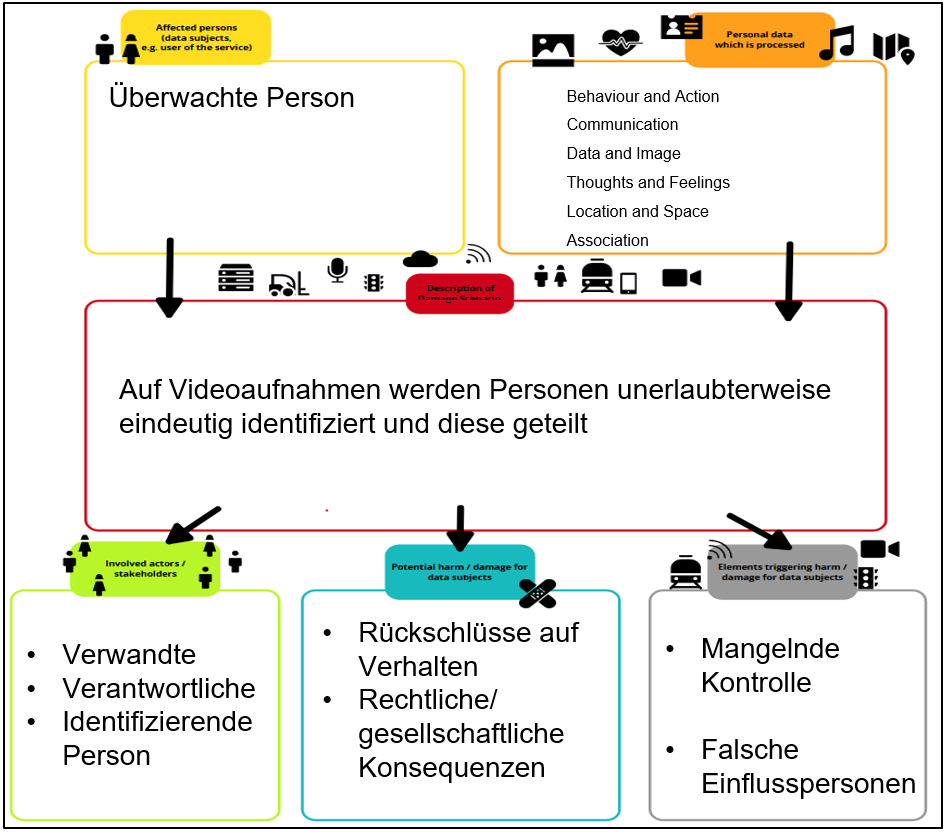
\includegraphics[width= 0.76\textwidth]{Bilder/privacy.png}
            \caption{Anwendung der Methode auf das konkrete Szenario}
            \label{fig:Privacy}
      \end{center}
\end{figure}
\newline
Direkt betroffen ist in dem Szenario die Person auf den Kamerabildern eindeutig identifiziert wurde. Alle gemäß Abschnitt \ref{abschnitt:7types} beschriebenen Aspekte können in diesem Szenario angewandt werden.
Stakeholder sind in dem Szenario das soziale Umfeld der Person, aber auch die Person die die Identifikation durchgeführt hat sowie deren Verantwortlichen. Der konkrete Schaden der entsteht, ist ein Rückschluss
der auf das Verhalten der Person zugelassen wird, aber auch rechtliche oder gesellschatliche Konsequenzen können nicht ausgeschlossen werden. Zu einem solchen Verstoß kann es durch mangelnde Kontrolle oder falsche
Einflusspersonen/ Vorgesetzte in dem Unternehmen kommen.

\subsection{Maßnahmen}
\label{abschnitt:massnahmen}
Maßnahmen können mittels der \glqq{}Privacy Design Strategies\grqq{} (PDS) abgeleitet werden \cite{Hoepman.2022}. Diese beschreiben Herangehensweisen, um Datenschutz zu gewährleisten.
Aus den möglichen Strategien ist die erste Maßnahme, den Fahrgast rechtzeitig über die Aufzeichnung zu informieren. Eine übliche Möglichkeit ist in Abbildung \ref{fig:hinweis} dargestellt, das Schild hängt im Eingangsbereich der Bahn
und auf auf der Internetseite findet sich ein Kontaktformular. Damit zusammenhängend sind die Strategien \glqq{}Enforce\grqq{} und \glqq{}Demonstrate\grqq{}. Wie in Kapitel \ref{abschnitt:konkret} beschrieben,
ist eine solche Art von Vorfall oft das Resultat durch ungenügenden Umgang mit Daten in der Unternehmenskultur. Nach einem Vorfall ist es entsprechend wichtig, ausgehend vom Management das Thema Datenschutz
stärker zu thematisieren. Dieses Vorgehen wird durch die PDS \glqq{}Enforce\grqq{} beschrieben. Damit einhergehend ist die Strategie \glqq{}Demonstrate\grqq{}, in welcher die getroffenen
Maßnahmen dokumentiert und nach außen präsentiert werden. Eine Kontrolle über die Daten gemäßs PDS \glqq{}Control\grqq{} kann in der Videoüberwachung allerdings nicht ermöglicht werden.

Neben den prozessorientierten PDS gibt es noch datenorientierte PDS. Eine anwendbare ist die PDS \glqq{}Hide\grqq{}. Diese beschreibt die Einschränkung des Zugangs zu den Videoaufzeichnungen durch Zugangsbeschränkungen
aber auch durch Verschlüsselung von Daten. Weniger anwendbar dagegen ist die PDS \glqq{}Separate\grqq{}. Diese beschreibt das kontextabhängige Aufteilen von Daten, um kein Schließen von Korrelationen zuzulassen.
Allerdings ist das Zuordnen der Kamerabilder zu den Orten oder Fahrzeugen essentiell. Auch das Minimieren und Abstrahieren von Daten ist nur schwerlich anwendbar, da eine Videoaufzeichnung versehen mit einem Zeitstempel
schon eine geringe Form der Datenerhebung darstellt.
\begin{figure}[ht]
      \begin{center}
            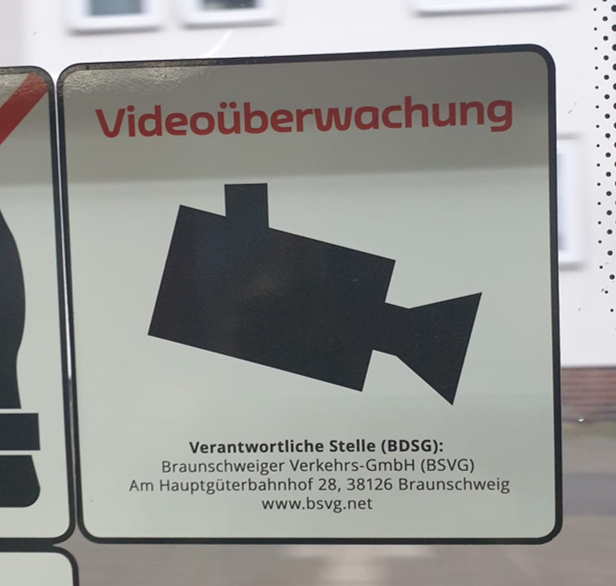
\includegraphics[width= 0.5\textwidth]{Bilder/hinweis.png}
            \caption{Hinweis in einer Straßenbahn der Braunschweiger Verkehrs-GmbH.\\Eigene Fotografie, 19.01.2023}
            \label{fig:hinweis}
      \end{center}
\end{figure}
